\documentclass{article}
\usepackage[margin=1in]{geometry}
\usepackage{graphicx}
\usepackage{listings}
\usepackage{xcolor}
\usepackage[T1]{fontenc}
\usepackage[utf8]{inputenc}
\usepackage{float}

\lstset{
    basicstyle=\ttfamily\small,
    breaklines=true,
    frame=single,
    language=C,
    keywordstyle=\color{blue},
    commentstyle=\color{green!50!black},
    stringstyle=\color{red}
}

\title{CS375 Assignment 7: Synchronization and Scheduling}
\author{Christian Clarke}
\date{\today}

\begin{document}
\maketitle

\section{Introduction}
This assignment focuses on thread synchronization using POSIX threads, mutexes, and condition variables. Each exercise demonstrates how to coordinate multiple threads, prevent race conditions, and enforce correct execution order.

\section{Exercise 1: Hello World}
\lstinputlisting{hello_world.c}

\textbf{Explanation:}  
The shared variable \texttt{hello} is protected by a mutex. The child thread increments it and signals the condition variable. The main thread waits until the value is updated before printing.

\textbf{Analysis:}  
Without synchronization, the second line could print first. The condition variable ensures correct ordering.

\begin{figure}[H]
\centering
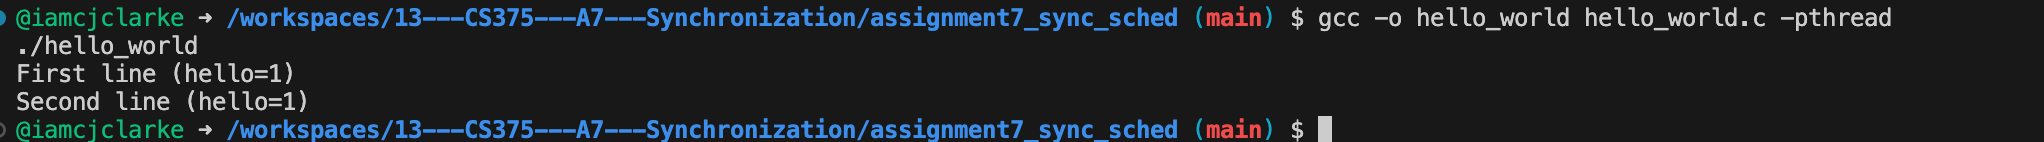
\includegraphics[width=\textwidth]{exercise1_screenshot.png}
\caption{Hello World output}
\end{figure}

\section{Exercise 2: SpaceX Problems}
\lstinputlisting{spacex.c}

\textbf{Explanation:}  
The counter thread decrements from 3 to 1 and signals when finished. The announcer waits for the countdown to reach 0 before printing.

\textbf{Analysis:}  
Prevents the announcement from printing early and ensures proper sequencing.

\begin{figure}[H]
\centering
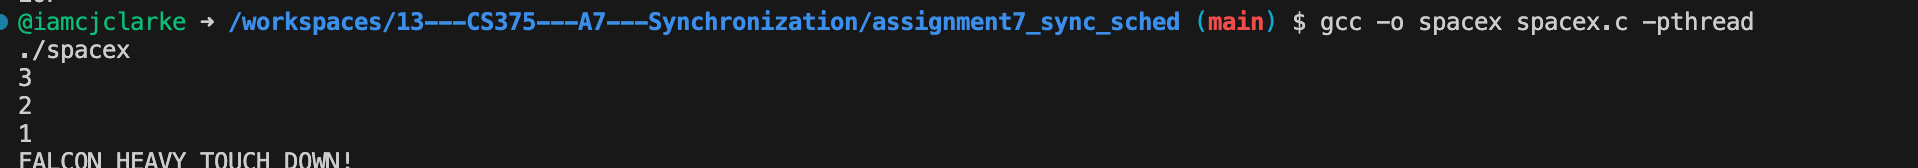
\includegraphics[width=\textwidth]{exercise2_screenshot.png}
\caption{SpaceX countdown output}
\end{figure}

\section{Exercise 3: I Love You, Unconditionally!}
\lstinputlisting{love.c}

\textbf{Explanation:}  
The helper thread updates the shared variable and signals the main thread.

\textbf{Analysis:}  
Condition variables prevent premature checks of shared data.

\begin{figure}[H]
\centering
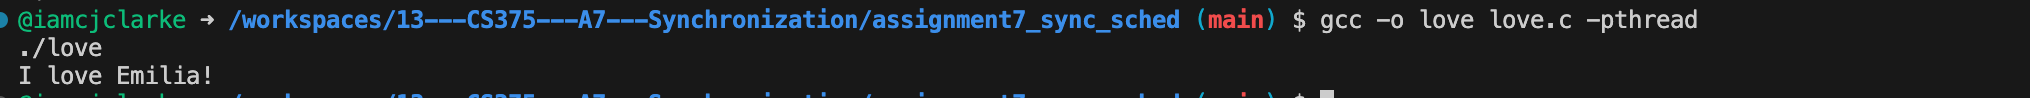
\includegraphics[width=\textwidth]{exercise3_screenshot.png}
\caption{Love program output}
\end{figure}

\section{Exercise 4: Locking Up the Floopies}
\lstinputlisting{floopy.c}

\textbf{Explanation:}  
Locks are acquired in a consistent order based on account ID.

\textbf{Analysis:}  
Prevents deadlock by removing circular wait conditions.

\begin{figure}[H]
\centering
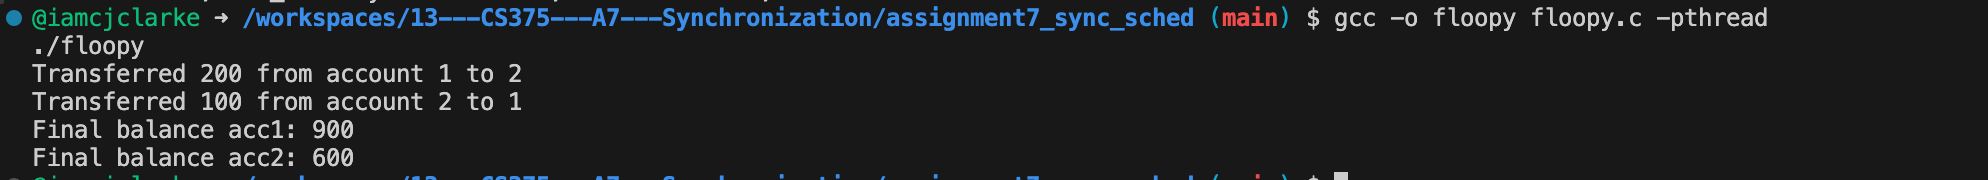
\includegraphics[width=\textwidth]{exercise4_screenshot.png}
\caption{Floopies transfer output}
\end{figure}

\section{Exercise 5: Baking with Condition Variables}
\lstinputlisting{baking.c}

\textbf{Explanation:}  
Threads coordinate batter, eggs, baking, and eating using condition variables.

\textbf{Analysis:}  
Ensures correct order: ingredients → bake → eat.

\begin{figure}[H]
\centering
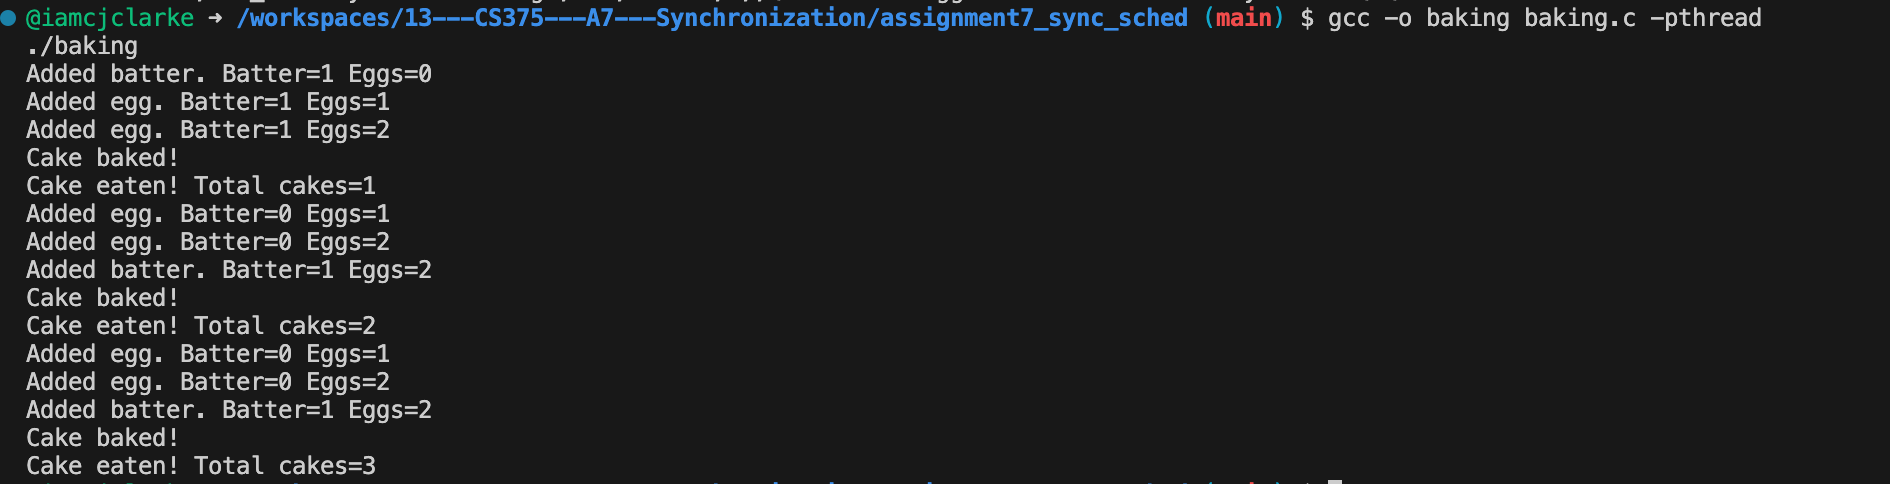
\includegraphics[width=\textwidth]{exercise5_screenshot.png}
\caption{Baking simulation output}
\end{figure}

\section{Exercise 6: Priority Donation}
\lstinputlisting{priority_transfer.c}

\textbf{Explanation:}  
Simulates priority donation by temporarily raising priority of locked resources.

\textbf{Analysis:}  
Helps reduce priority inversion.

\begin{figure}[H]
\centering
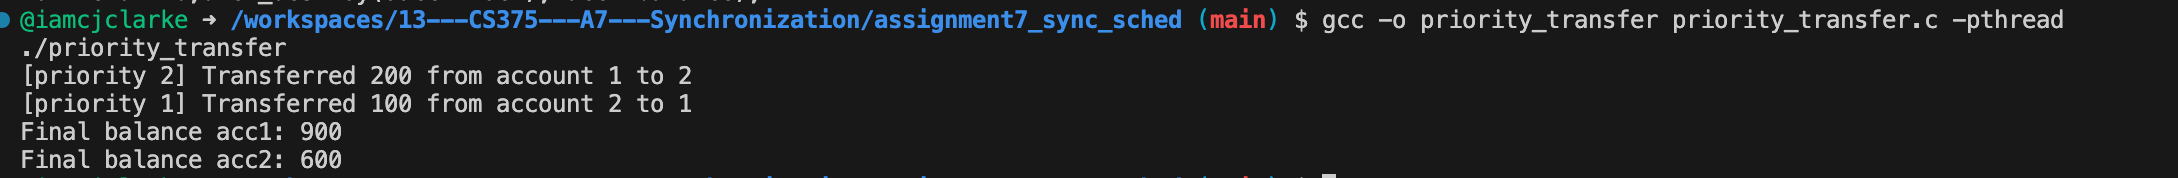
\includegraphics[width=\textwidth]{exercise6_screenshot.png}
\caption{Priority transfer output}
\end{figure}

\section{Exercise 7: Barrier Synchronization}
\lstinputlisting{barrier.c}

\textbf{Explanation:}  
Threads wait at a barrier until all arrive, then continue together.

\textbf{Analysis:}  
Guarantees synchronization across all threads.

\begin{figure}[H]
\centering
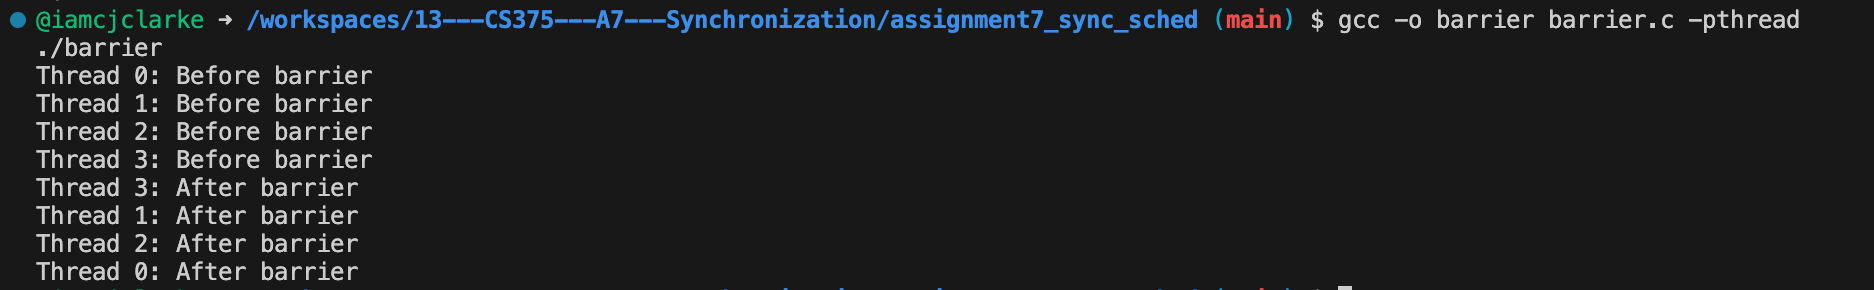
\includegraphics[width=\textwidth]{exercise7_screenshot.png}
\caption{Barrier output}
\end{figure}

\section{Exercise 8: Readers-Writers}
\lstinputlisting{readers_writers.c}

\textbf{Explanation:}  
Multiple readers allowed, but writers get priority.

\textbf{Analysis:}  
Prevents writer starvation while maintaining concurrency.

\begin{figure}[H]
\centering
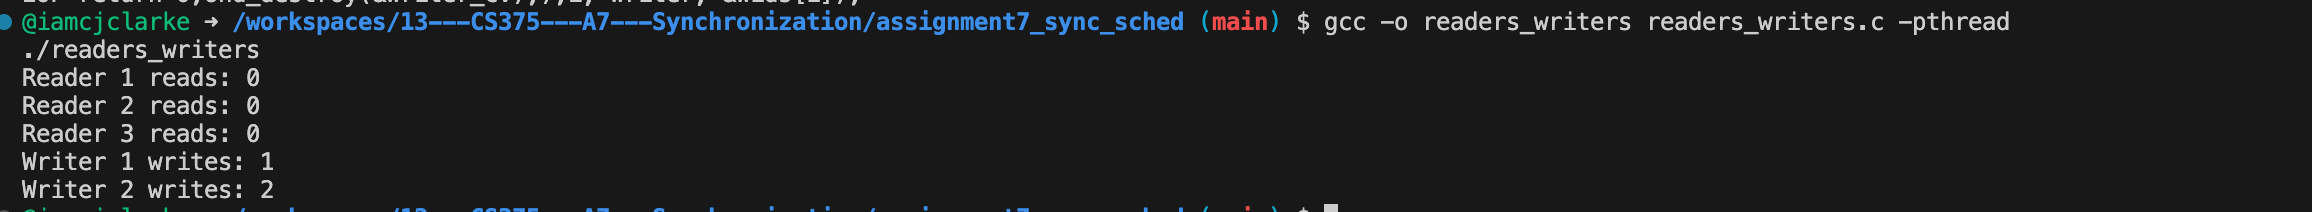
\includegraphics[width=\textwidth]{exercise8_screenshot.png}
\caption{Readers-Writers output}
\end{figure}

\section{Exercise 9: Thread Pool}
\lstinputlisting{thread_pool.c}

\textbf{Explanation:}  
A fixed pool of worker threads processes tasks from a shared queue.

\textbf{Analysis:}  
Improves efficiency by reusing threads instead of creating new ones.

\begin{figure}[H]
\centering
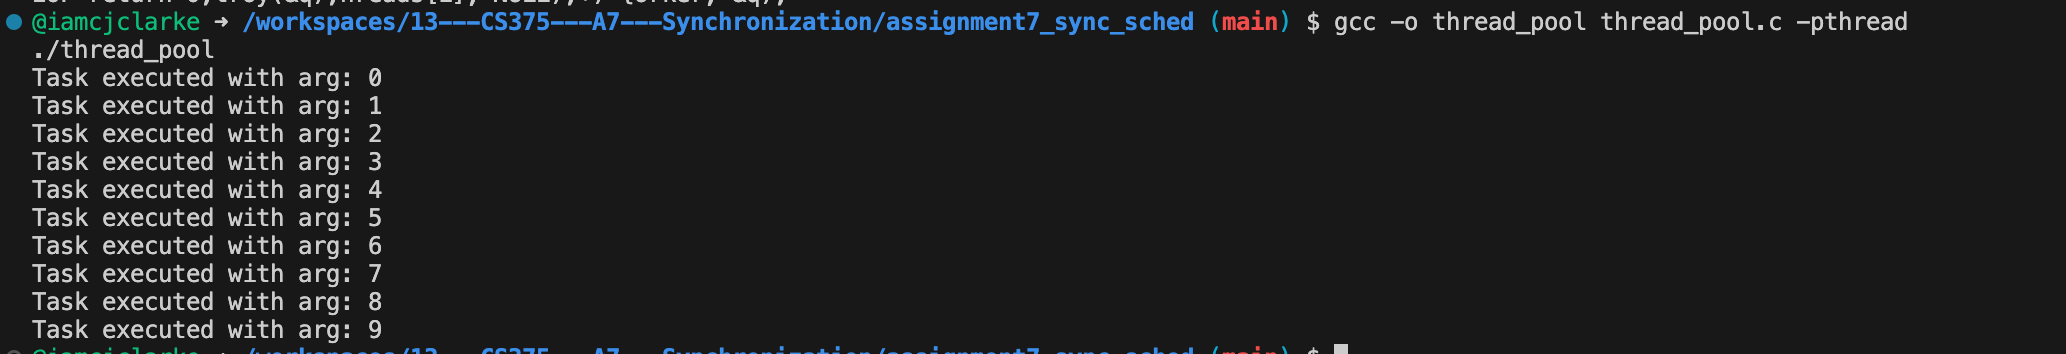
\includegraphics[width=\textwidth]{exercise9_screenshot.png}
\caption{Thread pool output}
\end{figure}

\end{document}
